\documentclass[english]{DESCARWINreport}

\usepackage{times}
\usepackage{helvet}
\usepackage{courier}
\usepackage{graphicx}
\usepackage{multirow}
%\usepackage[utf8]{inputenc}
\usepackage{algorithm}
\usepackage[noend]{algorithmic}
\usepackage{amsmath}
\usepackage{amsfonts}
\usepackage{amssymb}
\usepackage{array}
\usepackage{subfigure}
\usepackage{lscape}

%%%%%%%%%%%%%%%%%5 includepdf
\usepackage[final]{pdfpages}

\algsetup{indent=1.8em}
\renewcommand{\algorithmiccomment}[1]{// #1}
\newcommand{\pp}{planning tasks}
\newcommand{\PP}{planning task}
\newcommand{\dae}{{\em Divide-and-Evolve}}
\newcommand{\DAEI}{{\sc D\&E}}
\newcommand{\DAEII}{{\sc DaE2}}
\newcommand{\DAE}{{\sc DaE}}
\newcommand{\DAEX}{{\sc DaE$_{\text{X}}$}}
\newcommand{\DAEYAHSP}{{\sc DaE$_{\text{YAHSP}}$}}
\newcommand{\CPT}{{\sc CPT}}
\newcommand{\LPG}{{\sc LPG}}
\newcommand{\LAMA}{{\sc LAMA}}
\newcommand{\TFD}{{\sc TFD}}
\newcommand{\YAHSP}{{\sc YAHSP}}
\newcommand{\LAO}{{\sc LaO}}

\def\UU{{\mathbb{U}}}

%\title{DESCARWIN\\\bigskip {\em \LARGE The Marriage of Descartes and Darwin}\\\bigskip \bigskip \bigskip \bigskip \bigskip \bigskip \bigskip {\LARGE WP1: the \DAEX\ Planning System}}
\title{DESCARWIN\\\bigskip {\em \LARGE The Marriage of Descartes and Darwin}\\\vspace{8cm} 
{\LARGE D2.3\\
Experiments on on-line parameter control}}
\date{\today}
\laboratory{TRT - INRIA - ONERA}
\docref{62 441 217-179-1}

\revision{-}

\setlength{\parindent}{0cm}
\setlength{\parskip}{2ex plus 0.5ex minus 0.2ex}

\newcounter{hyp}
\setcounter{hyp}{1}
\newcommand{\hyp}{H\thehyp\stepcounter{hyp}}
\newcounter{defi}
\setcounter{defi}{1}
\newcommand{\defi}{D\thedefi\stepcounter{defi}}
\newcounter{con}
\setcounter{con}{1}
\newcommand{\con}{C\thecon\stepcounter{con}}

% Pour r�duire globalement l'espace entre les items d'une liste
% on peut �galement utiliser le bout de code suivant de M. Wooding
% Les param�tres utilis�s pour d�finir cette mise en page
% sont les suivants :
% \topsep espace vertical suppl�mentaire (ajoute � \parskip)
% 	ins�r� entre le texte pr�c�dant la liste et le 1er objet
% 	de la liste
% \partosep espace vertical suppl�mentaire ins�r� devant la liste
% 	si celle-ci est pr�c�d�e d'une ligne blanche
% \itemsep espace vertical suppl�mentaire (ajout� � \parsep)
% 	ins�r� entre les �l�ments d'une liste.

%%%% debut macro %%%%
% \makeatletter
% \toks@\expandafter{\@listI}
% \edef\@listI{\the\toks@\setlength{\parsep}{0pt}}
% \edef\@listI{\the\toks@\setlength{\topsep}{0pt}}
% \makeatother
%%%% fin macro %%%%


\begin{document}

\maketitle

%\cleardoublepage

\begin{revisions}
\begin{revtable}
\dates{APR. 13, 2011}{}{}{}
\writers{Matthias Brendel\\Johann Dr\'eo\\Mostepha Khouadjia\\Pierre Sav�ant\\Marc Schoenauer\\Vincent Vidal}{}{}{}
\approvers{P. Sav\'eant}{}{}{}
\end{revtable}
\begin{revisionlabels}
\revlabel{initial version}
\revlabel{}
\end{revisionlabels}
\end{revisions}

\begin{abstract}
This deliverable does not exactly match its initial description that had been made in the original Description of Work of the DESCARWIN proposal. It turned out indeed that the methods that we had in mind when writing the proposal couldn't work in the framework of AI planning as approached with DaE, due to the very small number of different fitness values encountered during DaE runs. This will be detailed in the first Chapter 2 of this deliverable. \\

On the other hand, the Learn-and-Optimize framework (as described in Deliverable 2.2, Chapter 2) can be thought of as an intermediate method between off-line and on-line learning: if the optimizer is installed in some production line, and has to solve a sequence of instances of the same domain, then the instance-based method Learn-and-Optimize is a way to adjust the parameters of the optimizer to the current instance automatically, without any human intervention, i.e., at runtime. A lot of efforts were devoted to further developments of the LaO method \ldots that turned out however to fail to improve the initial results. Furthermore, this was confirmed when LaO was submitted to the IPC'7 competition, where unfortunately it obtained rather poor results - in part only because of the lack of time for preparation before the post-doc in charge, Matthias Brendel, left the project. This is detailed in Chapter 3, and a copy of the short paper that was required to present the candidate planners for the competition is appended.\\

Also, and as planned in the original workplan, our effort had to turn to the multi-objectivization of Divide-and-Evolve, and of course this also includes adapting the parameter tuning methodology to the multi-objective context. It also turned out that a new framework for off-line parameter tuning, called ParamILS (see reference [XXX] in Chapter 4), developed at University of British Columbia, was gaining popularity, because of the excellent ratio (performance / CPU cost) it obtained compared to the Racing procedure that we had been using up to then (described in Chapter 1 of Deliverable 2.1). We hence decided to modify our off-line tuning method and to exclusively use ParamILS further on. Details of ParamILS and our implementation are briefly given in Chapter 4.\\

As mentioned above, the new framework was initially set up for the multi-objective work on DaE, and one issue that had not been planned ahead arose: which metric use within ParamILS to assess the performance of the different parameter sets? For the Pareto-based multi-objective algorithms, the Hypervolume was an obvious candidate, and it turned out it performed very well indeed. But for the aggregation approach, in which a single-objective DaE is used to optimize a weighted sum of the objectives, the obvious choice was to use, for each of the runs optimizing a weighed sum of objectives, the very same fitness, i.e., the very same weighted sum. However, it turned out that a better choice was to also use the hypervolume indicator, even though different from the metric that each run optimizes, as demonstrated in Chapter 5. 

As a matter of fact, this work was published as ``Khouadjia, M. , Schoenauer, M. , Vidal, V. , Dr�o, J. and Sav�ant, P.. Quality Measures of Parameter Tuning for Aggregated Multi-Objective Temporal Planning. In Panos Pardalos and Guiseppe Nicosia, eds.: LION'7 -- 7th Learning and Intelligent OptimizatioN Conference, Springer Verlag, LNCS : To appear. Catania, Italy. January 2013.''

A copy of the published paper is included after a brief recall of the context and main results, in Chapter 5.



\end{abstract}

\tableofcontents

% \newpage
% 
% \chapter{Introduction}

\newpage
\chapter{Failure of on-line control methods based on operator reward}

When the DESCARWIN proposal was written, we had a clear idea in mind regarding on-line parameter control (see Deliverable 2.1 for the list of the now-standard vocabulary): because the INRIA partner had been involved in several works regarding on-line parameter control, we anticipated that the same approaches could be used within \DAE\ framework. In particular, this concerned the on-line parameter control, where the parameters are modified during the run, depending on the history of the search, the idea was to port Adaptive Operator Selection (AOS) methods, for which the INRIA partner had a large expertise (PhD thesis of Alvaro Fialho entitled {\em Adaptive Operator Selection for Optimization} and defended in December 2010).

The basic idea of AOS methods (see Deliverable 2.1, Chapter 4) relies on two components: whenever an operator is applied, its impact is recorded, and some {\em reward} is given to the operator, usually based on the fitness improvement, i.e., depending whether the fitness of the offspring is better than that of the parent(s). The second component is a decision mechanism that uses the past rewards of all operators to decide which one to use next. There are several such decision mechanisms, e.g. Probability Matching, Adaptive Pursuit, and the family of Multi-Armed bandit based methods developed by Alvaro Fialho in his PhD. But all of them are based on some reward that is computed from the fitness improvement brought by the operators - and such rewards are zero if the fitness does not increase in the population. Note that this is true even for the rank-based mechanism that is described in detail in Chapter 4 of Deliverable 2.1, rank-based mechanism that was our preferred candidate AOS for \DAE\ because of its invariance by monotonous transformation of the fitness, and is hence independent of any fitness scaling, the Achille's heel of most AOS method based on fitness improvement.

\begin{figure}[h!]
\begin{center}
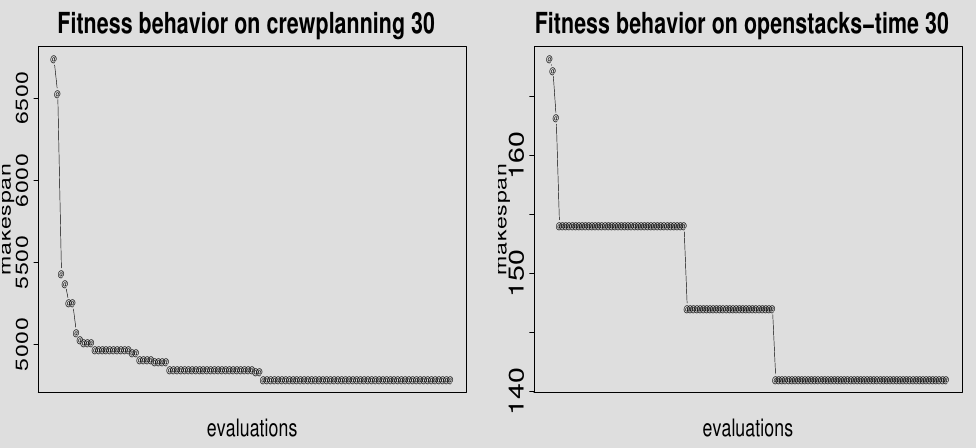
\includegraphics[width=0.9\textwidth,height=6cm]{fitnessBehavior.png}
\end{center}
\end{figure}


During \DAE\ runs, however, it turned out that very few fitness improvements do take place -- mostly because there are very few possible fitness values, at least when reaching regions of the search space around the optimum. Figure \ref{fig:fitnessImprovement} displays typical evolution of the best fitness in the population during two \DAE\ runs, for two large instances of two different IPC domains, {\tt crewplanning} and the temporal {\tt openstack}: the best fitness in the population goes through only 3 values for {\tt openstack}, and less than a dozen for {\tt crewplanning}. There is hence little hope that AOS based on fitness improvement (even, as said above, the champion rank-based AOS) can learn which operators perform best with so few example of improving operations.

After some preliminary experiments that confirmed this trend, it was decided to 
\begin{enumerate}
 \item not waste any more time trying to run some Adaptive Operator Selection method to \DAE\ context
 \item investigate the {\em Learn-and-Optimize} (\LAO) approach that had been developped with M�ty�s Brendel within the project; Indeed, \LAO\ can be seen as a somehow intermediate method between off-line and on-line method, as it learns how to predict the best parameters from solved instances (hence off-line), but later determines the optimal parameters for new and unseen instances: this is done automatically, if not during the run -- and at least a single run is needed for each new instance, by contrast to pure off-line method who require many runs to adjust the parameters for any instance.
 \item put more efforts on the multi-objective case, because the topic was gaining interest in the AI Planning community (again -- see Deliverable 3.3). And it turned out that indeed some more efforts were needed for off-line parameter setting when going from single- to multi-objective contexts.
\end{enumerate}
The rest of the deliverable will thus detail the work done on \LAO\ following the preliminary work that has been introduced in Deliverable 2.2, Chapter 3, that unfortunately didn't bring much improvement over the preliminary results. Then we will turn to the specific work done in the context of Pareto-based multi-objective optimization, in relationship with Deliverable 3.3.

\newpage	
\chapter{Further work on \LAO}

\section{Improvements}

After the very promising first results of the Learn-and-Optimize framework, published in GECCO (as a poster) and the Evolution Artificielle conference (

Several research directions have been explored to improve the results of the Learn-and-Optimize framework, that alas didn't provide significant improvement on the AI Planning domains, and hence have not lead to any publication -- as unfortunately nowadays in science, negative results
are no results to publish.

These directions regard on the one hand the features are used to characterize the different instances. In the published results, the same initial 12 features have been introduced and used. But we suspect that these original 12 features are not sufficient to capture the peculiarities of the instances w.r.t. the parameters of the planner. Indeed, adding new features is a way to increase the chances to be able to identify relevant characteristics, and derive an accurate model to predict some good values for the parameters; however, the more features the higher the chances to hinder the learning phase with useless information, eventually hiding the correct correlation and resulting in worse results.

Note that, even though they didn't improve the results, these features are in the code delivered as D2.4.

Two sets of possible interesting features have been explored.

\begin{itemize}
\item Beyond the 12 initial features, we developed statistical features of the "histogram type``, e.g., the chronopartition, number of types and number of terms. All these features result in a histogram, i.e. a series of numbers, which can be interpreted as a distribution. For each of these, we computed the mean, the median, and the value at the first and third quartile. Using them either alone or in addition to the initial 12 features did not improve the results with independent tests. 

\item Furthermore, we also developed the probing features, i.e., running a naive heuristic (e.g., greedy, depth first, \ldots) for a short time and recording the improvements. Using such features, again, did not improve the results. None of these features harmed a lot, but one could nevertheless see some degradation of the results -- which is why this line of research was abandoned. In spite of the fact tests with the additional features 24 or 32 features were made on around 100 instances, we thought that there was no risk of over-fitting. However, it seems there was a slight over-training, as the results on the test set were worse,whereas the results onthe training set were slightly improved. But the main problem was of course that these new features were not useful at all.
\end{itemize}

On the other hand, we investigated an indirect approach to the model XXX
\begin{itemize}

\item  We developed the indirect model with Artificial Neural Networks. The indirect model was optimized using CMA-ES algorithm when it was queried for new parameters. However, this approach resulted in a decrease  of around 0.8 in ratio compared to the default parameters.

Also we tried an indirect model using Rank-SVM regression. Here, after optimizing only in a small neighborhood around the default parameters, the decrease (a ratio with defaults parameters) was slightly bellow 1. So, the indirect models did not really work out.

\item A worrying issue is that of generalization: a model trained for one domain was never good enough for another domain. We also tried to train a big, domain-independent model using all of the IPC-6 domains, meaning that we were using more than 500 instances for training. This did not work with an independent test, again the ratio was around 0.8. So learning a model more general than one domain seems to be much harder. 

\end{itemize}

\section{Lao at IPC11}

\newpage
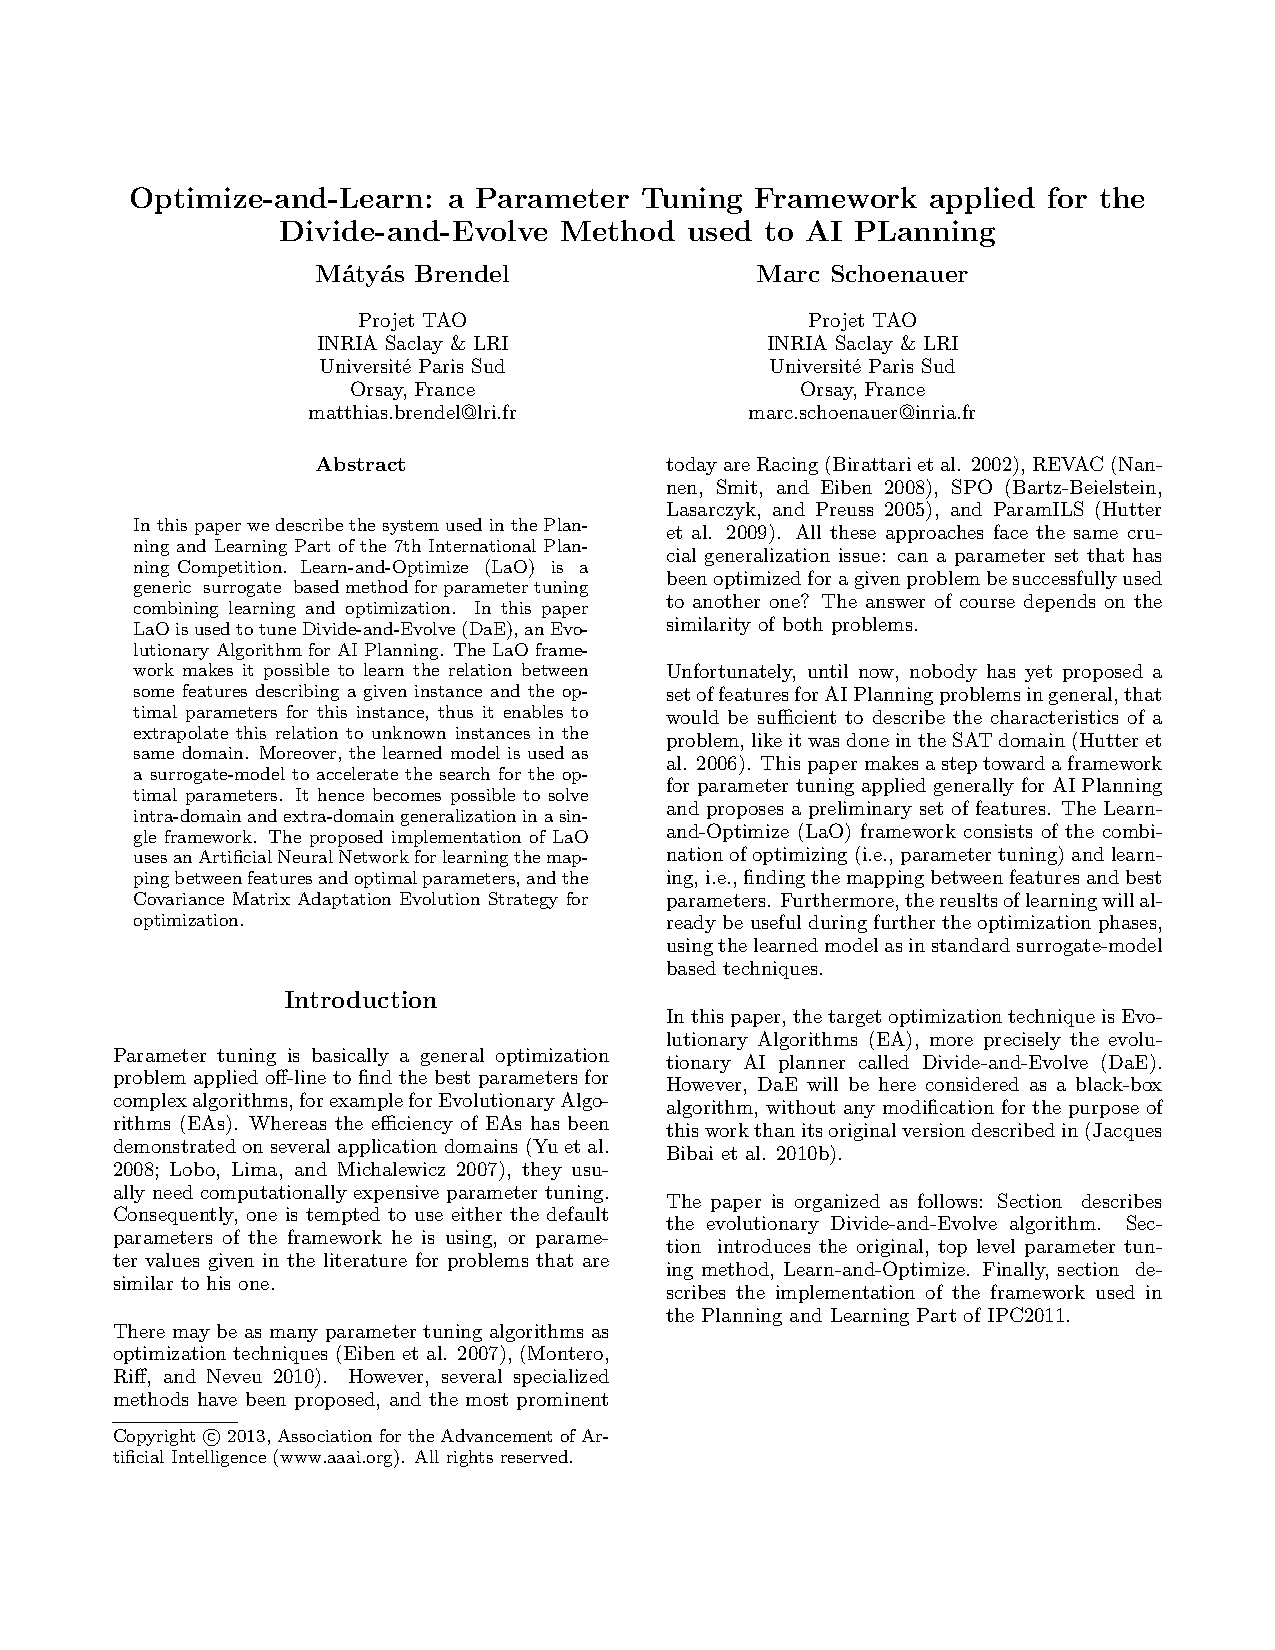
\includepdf[height=30cm,pages=-,offset=2.2cm -4cm]{ipc2011.pdf}
\newpage

\chapter{A new framework for off-line tuning: ParamILS}

It is widely acknowledged today that off-line parameter tuning has somehow reached a mature state, and is considered a mandatory step when evaluating and validating the performance of any optimization or machine learning algorithm. This recent trend, advocated by Holger Hoos (University of British Columbia) under the name of {\em Programming by Optimization} (see e.g., http://www.prog-by-opt.net/ and references herein) has however been started many years ago in the Evolutionary Computation community, with the seminal work {\em  Parameter control in evolutionary algorithms} by A.E. Eiben, R. Hinterding, and Z. Michalewicz published in the IEEE Transactions on Evolutionary Computation (3(2):124-141) in 1999, and the many different (meta-)algorithms that have been proposed in that respect (see Deliverable 2.1, Section 3.3.2 for detailed descriptions). However, the situation seems to have slightly evolved since this Deliverable was written, and whereas all our past experiments were using some Racing procedure, the ParamILS framework developed at University of British Columbia was found better performing, and more flexible and general purpose tool than all EC-specific approaches (like SPO and REVAC for instance), and than the F-Race framework proposed by IRIDIA. 


\newpage
\chapter{Using ParamILS for multi-objective parameter setting: the case of the aggregation approach}


\newpage
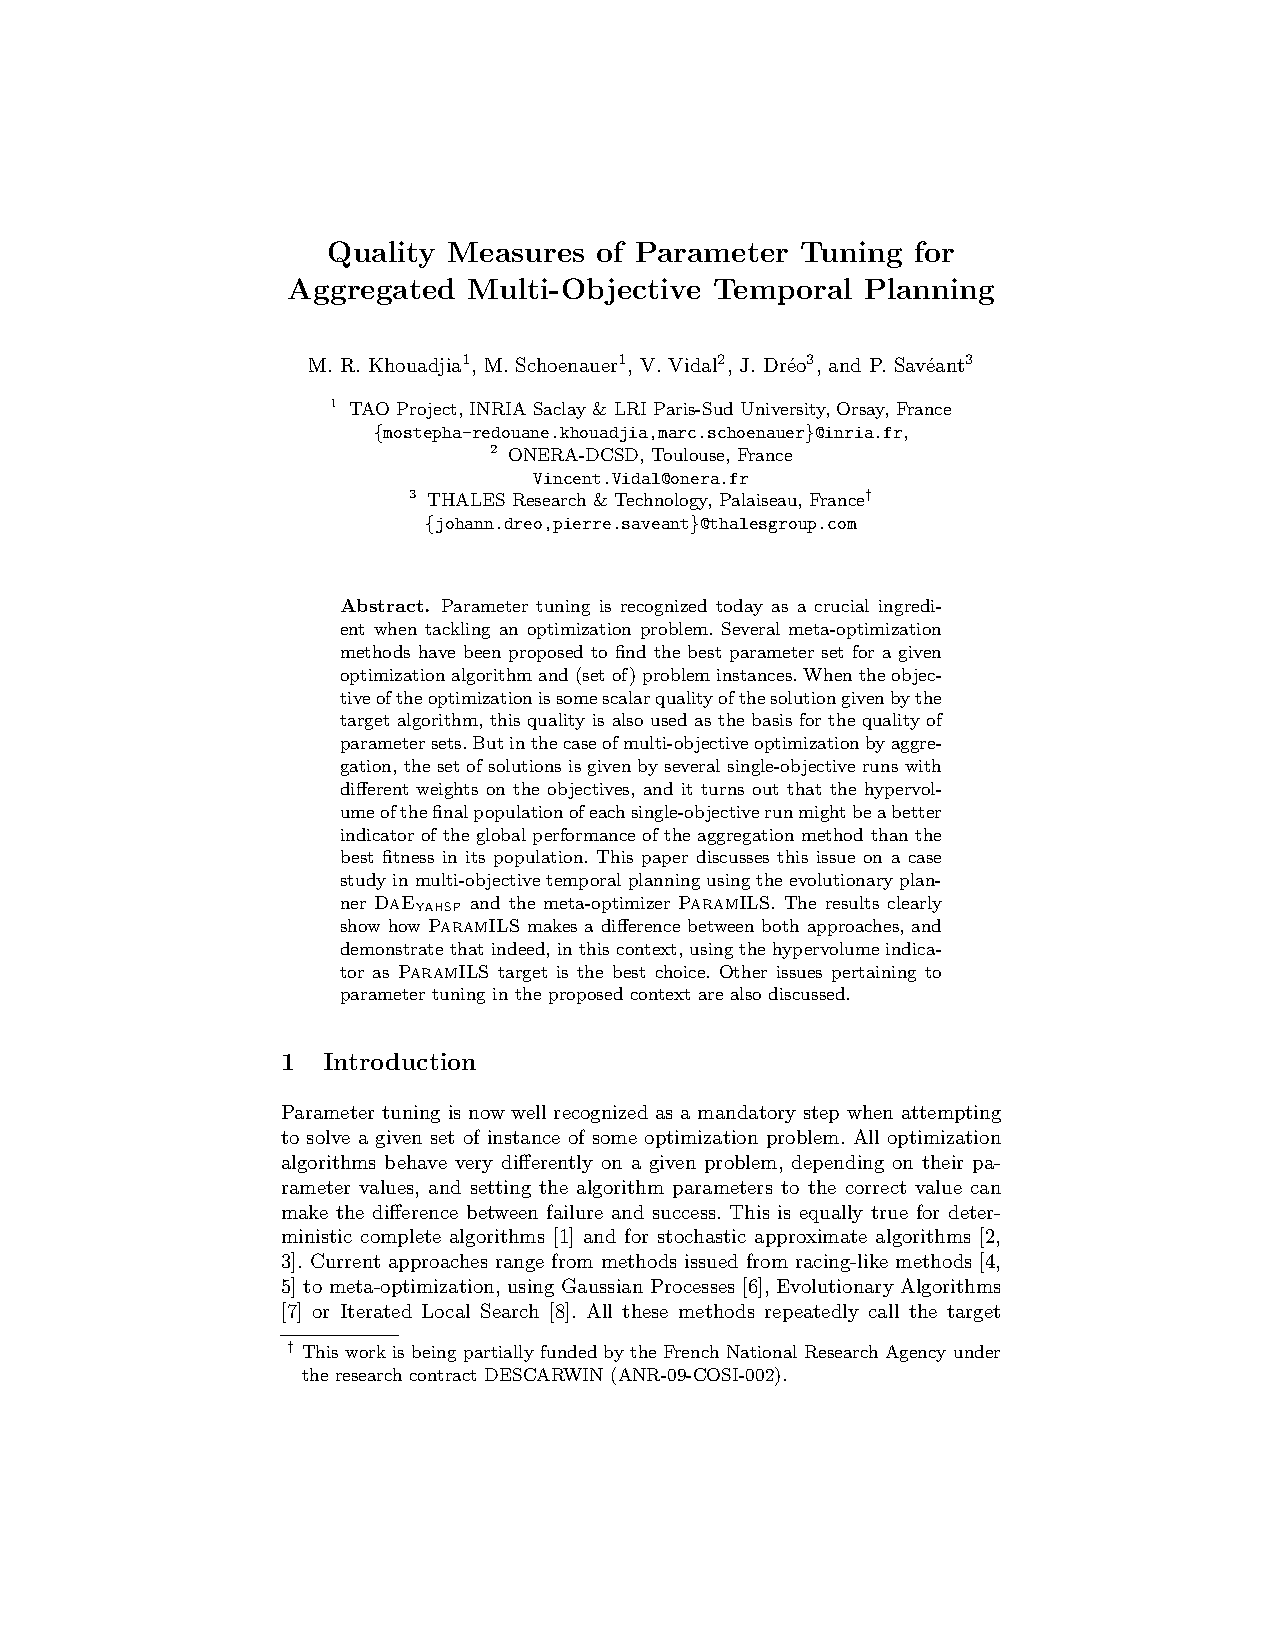
\includepdf[height=32cm,pages=-,offset=2.2cm -4cm]{lion_final.pdf}
\newpage



% \chapter{Conclusion}
% \label{conclusion}


% \chapter{References}
% \bibliographystyle{alpha}
% \bibliography{xxx}

\end{document}

%%%%%%%%%%%%%%%%%%%%%%%%%%%%%%%%%%%%%%%%%%%%%
Rapport de r�sultats de Matthias en vue IPC 2011 ?????

Section \ref{section:competition} describes the special settings of our system used in the competition. Finally, Section \ref{section:future} gives some pointers to future plans and work.  


\section{The IPC Competition}
\label{section:competition}

In the Planning and Learning Part of IPC2011 (IPC), there were 5 domains published, with a corresponding problem-generator for each domain. The 5 domains are Ferry, Freecell, Grid, Mprime, and Sokoban. We generated approximately 100 instances for each domain, since this seemed to be appropriate for a running time of 2-3 weeks. The description of the track fixes running time as 15 minutes. Since we use number of evaluations as a terminating criterion, we carried out a run for each instances on our own server to measure the median of number of evaluations for each instance with our default parameters. The median of 11 runs were taken and used as a termination criterion for each instance in the train set. For many instances we did not have any result in 15 minutes, those we had to drop. The remaining instances were used for training. 

 \begin{table*}[ht]
\centering
\begin{tabular}{l c c c c c c}
\hline\hline
Name & \# of iterations & \# of training instances &  ANN-error & quality-ratio LaO& quality-ratio ANN \\ 
\hline
Ferry & 12 & 32 & 0.17 & 1.06 & 0.59   \\
Freecell& 12 & 108 & 0.08 & 1.09 & 1.05   \\
Grid & 9 & 55 & 0.09 & 1.09 & 1.0   \\
Mprime & 8 & 64 & 0.16 & 1.11 & 1.01 \\
Sokoban & 8 & 32 & 0.11 & 1.22 & 0.79  \\
\hline
\end{tabular}
\label{table:domains}
\caption{Domains: note that only the actually usable training instances are shown. ANN-error is given as MSE, returned by FANN}
\end{table*} 

\begin{table*}[ht]
\centering
\begin{tabular}{l c c c}
\hline\hline
Name & Minimum & Maximum & Default value \\ 
\hline
Probability of crossover & 0.0 & 1 & 0.8 \\
Probability of mutation & 0.0& 1& 0.2 \\
Rate of mutation add station& 0& 10& 1 \\
Rate of mutation delete station& 0& 10& 3 \\
Rate of mutation add atom& 0& 10& 1 \\
Rate of mutation delete atom& 0& 10& 1 \\
Mean average for mutations& 0.0& 1& 0.8 \\
Time interval radius& 0& 10& 2 \\
Maximum number of stations& 5& 50& 20 \\
Maximum number of nodes& 100& 100000& 10000 \\
Population size& 10& 300& 100 \\
Number of offsprings& 100& 2000& 700 \\
\hline
\end{tabular}
\label{table:parameters}
\caption{Controlled Parameters}
\end{table*} 

Table \ref{table:domains} shows the data for each domain, as you can see from the approximately 100 instances from each domain we could only use all instances in the domain Freecell. In the other domains we got much less usable instances. The Mean Square Error (MSE) is shown for each domain. Note that since there can be multiple optimal parameters for the same instance (fitness-function is discrete), there might be an unavoidable error of the ANN.

5 iterations of CMA-ES were carried out, followed by one ANN and one gene-transfer, and this cycle were iterated in the algorithm. This means that for example CMA-ES was running for 50 iterations for the Grid domain.

The ANN had 3 fully connected layers, and the hidden layer had the same number of neurons as the input. Learning was done by the conventional back-propagation algorithm, which is the default in FANN. The ANN was only trained for 50 iterations in one iterations of LaO, so that we avoid over-training. Over the 10 iterations of LaO this means that 500 iterations of the ANN was carried out.

Termination criterion in the competition was simply the available time, the algorithm was running for several weeks parallel on our cluster, which is used also for other research, i.e. only a small number of 4 or 8-core processors were available for each domain in average.

The parameters of DAEx controlled are described in table \ref{table:parameters}. For a detailed description of these parameters, see \cite{BibGECCO:2010}. The feature set consists of the number of fluent, goals predicates objects and types in the domain or instance, respectively. One further feature is called mutex density, which is the number of mutexes divided by the number of all fluent-pairs. We also added number of lines, words and byte-count - obtained by the linux command called "wc" - of the instance and the domain file as some not so serious, primitive features.

\section{Future Work}
\label{section:future}	

Since LaO is only a framework, as indicated other kind of learning methods, and other kind of optimization techniques may be tried. Also the benefit of gene-transfer and/or cross-over might be investigated further. One shall also test, how inter-domain generalization works. Maybe it is possible to learn a mapping for all the domains, since the features may grasp the specificity of a domain. Naturally, the set of features may always be extended, or tested. Feature-selection would become important only if data with a considerable number of features and instances are present. This is not the case yet.
